\documentclass[11pt,journal]{article}
%\usepackage{hyperref}
%\usepackage[breaklinks]{hyperref}
\usepackage{breakurl}
\usepackage{url}
\usepackage{listings}
\usepackage{courier}
\usepackage{amsmath}
\usepackage{graphicx}
\graphicspath{ {/home/agata/Documents/coursework/SensorNetworks/Project/} }
%\ifCLASSOPTIONcompsoc
% IEEE Computer Society needs nocompress option
% requires cite.sty v4.0 or later (November 2003)
\usepackage[nocompress]{cite}

%\else
% normal IEEE
\usepackage{cite}
%\fi

\hyphenation{op-tical net-works semi-conduc-tor}
\addtolength{\oddsidemargin}{-.875in}
\addtolength{\evensidemargin}{-.875in} 
\addtolength{\textwidth}{1.75in}

\addtolength{\topmargin}{-.875in}
\addtolength{\textheight}{1.75in}
\newcommand\tab[1][1cm]{\hspace*{#1}}
\begin{document}
	\title{Sensor Networks and Mobile Data Communication, Project Report}
	
	\author{UID: 1690550}% <-this % stops a space
		%\protect\\
		%\thanks{}}
	
	% The paper headers



	% IEEEtran.cls defaults to using nonbold math in the Abstract.
	% This preserves the distinction between vectors and scalars. However,
	% if the journal you are submitting to favors bold math in the abstract,
	% then you can use LaTeX's standard command \boldmath at the very start
	% of the abstract to achieve this. Many IEEE journals frown on math
	% in the abstract anyway. In particular, the Computer Society does
	% not want either math or citations to appear in the abstract.
	
	% Note that keywords are not normally used for peerreview papers.
	
	% make the title area
	\maketitle
	
	
	% To allow for easy dual compilation without having to reenter the
	% abstract/keywords data, the \IEEEcompsoctitleabstractindextext text will
	% not be used in maketitle, but will appear (i.e., to be "transported")
	% here as \IEEEdisplaynotcompsoctitleabstractindextext when compsoc mode
	% is not selected <OR> if conference mode is selected - because compsoc
	% conference papers position the abstract like regular (non-compsoc)
	% papers do!
	%\IEEEdisplaynotcompsoctitleabstractindextext
	% \IEEEdisplaynotcompsoctitleabstractindextext has no effect when using
	% compsoc under a non-conference mode.
	
	
	% For peer review papers, you can put extra information on the cover
	% page as needed:
	% \ifCLASSOPTIONpeerreview
	% \begin{center} \bfseries EDICS Category: 3-BBND \end{center}
	% \fi
	%
	% For peerreview papers, this IEEEtran command inserts a page break and
	% creates the second title. It will be ignored for other modes.
	%\IEEEpeerreviewmaketitle
	\section{Introduction}
	The simulated problem involves a delay-tolerant network (DTN), with two stationary nodes 0 and 2, positioned 10000 m apart, and a mobile node 1, moving between them, starting from (0,3) in the x-y plane. The initial position of the nodes are shown in Fig. 1. We introduce the movement later; for now Node 1 is stationary.
	
	\begin{figure}[h]
		\centering
		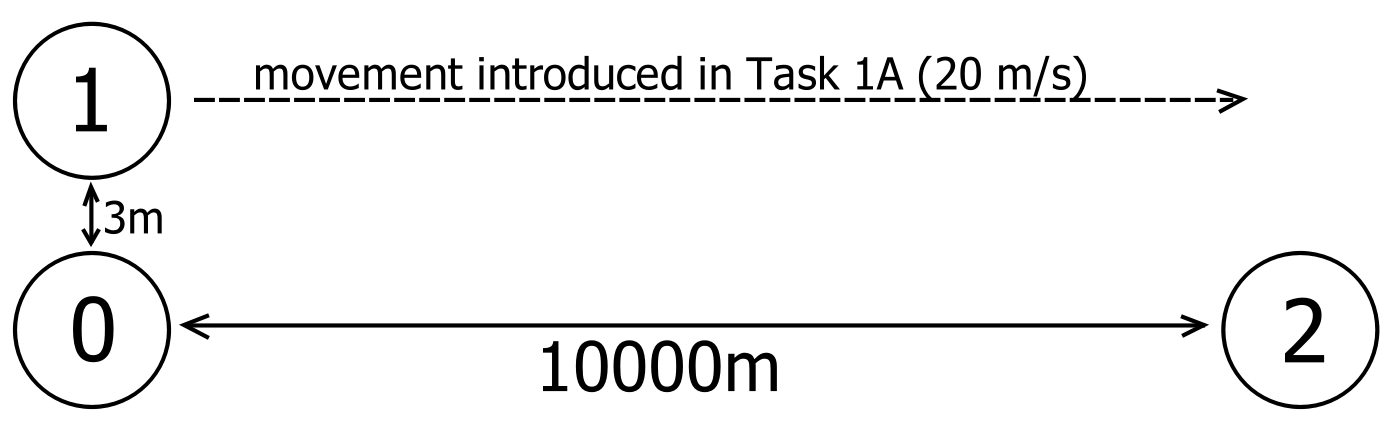
\includegraphics[]{project_topology1.png}
		\caption{Initial topology of the network, with the movement as introduced in the first task}
	\end{figure}

	\subsection{Node 0}
	The code responsible for Node 0 (first village) behaviour starts at line 234 of the original code. 
	
	The function \texttt{Node0DataGen()} maintains the buffer with the messages. It calls itself every second. With each call, it increases the \texttt{global\_counter} variable which acts as a stamp for the mails, and adds the message to the buffer, by updating the head. If adding the message to the buffer would exceed the buffer size, it also moves the tail forward. On the other hand, if the buffer is empty, it also marks the \texttt{isbufferempty} flag as non-empty after adding a message to the buffer. In this case, the tail and head are set to 1.
	
	Sending the messages to Node1 (the bus) is done by \texttt{Node0SendPacket(...)} function. It tries to send the buffer from Node0 every 0.25 seconds. The encapsulation of the buffer is done by creating a \texttt{MyHeader} object. It contains the following pieces of information:
	
	\begin{itemize}
		\item packet type, which here is always 1 for data
		\item \texttt{isbufferempty} - the flag indicating that the buffer is empty. Given that this is performed within an if statement, only if the buffer contains messages, this value should always be 0.
		\item \texttt{head} - head of the buffer
		\item \texttt{tail} - tail of the buffer
	\end{itemize}

	The \texttt{MyHeader} is then put into a packet and sent. If the buffer is empty, instead of creating a \texttt{MyHead} we just log that there is nothing to send.
	
	Finally, whenever Node0 receives an acknowledgement from Node1 that it got the packet with messages, it clears the buffer by setting \texttt{isbufferempty} to 0.
	
	\subsection{Node 1}
	The code describing Node1's behaviour starts at line 298. It has three functions, \texttt{Node1ReceivePacket(...)}, \texttt{Node1AckLoop(...)},and \texttt{Node1SendPacket(...)}. 
	
	The \texttt{Node1ReceivePacket(...)} picks up packets sent by Node0. If it's a data packet, it copies the packet's content into its own buffer, and sets \texttt{Node1SendAck} flag to 1. If it's not a data packet, then it is an acknowledgement from Node 2, which gets logged.
	
	When \texttt{Node1SendAck} flag is set to 1, the \texttt{Node1AckLoop(...)}function, running every 0.01 s, sends the acknowledgement, unsets the \texttt{Node1SendAck} and sets the \texttt{Node1Pending} flag to 1. Finally it schedules the packet to be sent to Node2.
	
	Once the acknowledgement is sent, \texttt{Node1SendPacket(...)} begins its attempts to send the packet to Node2, in 0.25 s intervals. It copies information stored in its buffer to a packet and tries sending it.
	
	\subsection{Node 2}
	
	Node2's role is to receive packets from Node1 and acknowledge it. Starting at line 373, the receiving of packets is covered by function \texttt{Node2ReceivePacket(...)}. It extracts the information from the header and stores them in local variables. Of a particular note is the \texttt{Pkt\_no\_last\_seen\_by\_node2}. It keeps track of the last received packet by storing the stamp of the last message in the previous packet. If the arriving packet contains a message with a newer stamp, Node2 updates its records, and logs the values from the header. Finally it marks \texttt{Node2SendAck}, which will then be used to prompt an acknowledgement.
	
	\texttt{Node2AckLoop(...)} runs at 0.01 s intervals. Every time it creates a packet, however it is sent only if \texttt{Node2SendAck} is marked as 1 by the previous function, after being set to type 0 for ack (cf. 1 for data). This function also logs that the acknowledgement is sent, and marks \texttt{Node2SendAck} back to 0.
	
	\subsection{Overall behaviour}
	
	All nodes are set to unicast mode, with Node0 connected to Node1, and Node1 connected to Node2. They all follow the 802.11 standard, and adhere to AODV protocol with route timeout of 10 min. Note that this is longer than the simulation, which runs for 500 s. The transmission power remains constant at 1.5 dBm throughout the simulation. 
	
	\subsection{Propagation Loss Model}
	
	The propagation loss model is constant range, which means that up to the given maximum distance (200 m initially) the packets are transmitted with the given transmission power (1.5 dBm in this case). Beyond the maximum range, the transmission power drops to -1000 dBm, which is effectively 0\cite{range loss doc}. Note that with Node1 travelling along the $y=3$ line, it means that it needs to be at $x \leq 199.98 \approx 200$ to reach Node0, and at $ x > 9800$ to reach Node2.
	
	\section{Methods}
	\subsection{Task 1A}
	To introduce movement of Node1, we first add \texttt{"ConstantVelocityMobilityModel"} using the Mobility Helper that already exists in the code. It is done by adding the following line at line 476:
	
	\texttt{mobilityMobileNode.SetMobilityModel("ns3::ConstantVelocityMobilityModel");}
	
	
	After installing the Mobility Helper, we explicitly set the velocity of Node1, by:
	
	\texttt{(mobileNode.Get(0) -> GetObject<ConstantVelocityMobilityModel>()) -> SetVelocity (Vector(20.0, 0.0, 0.0));}
	
	This is a much more certain way of setting the velocity of the node, than setting it as an attribute while setting the Constant Velocity Mobility Model, which sometimes may not be parsed correctly.
		
	Note that with the transmission range of 200 m, even with Node1 moving, its buffer gets overwritten multiple times, before it is out of range of Node0.
	
	To work out the maximum distance between Node0 and Node1 for a given speed of Node1, we iterate over Node1's speeds, ranging from 20 to 200 m/s, at 10 m/s intervals, and over distances, ranging from 3 to 300 m. We do not expect to see anything at a range exceeding 200 m because of the propagation loss model. 
	
	In each iteration, we calculate the duration of the simulation by the following formula:
	
	\[\text{duration} = \dfrac{\text{Distance between Node0 and Node1}}{\text{speed of Node1}} + 10\]
	
	We add 10 at the end to make sure that Node1 goes past the x coordinate of Node2.
	
	Our findings are summarised in the graph in Fig 2.
	
	\begin{figure}[h]
		\centering
		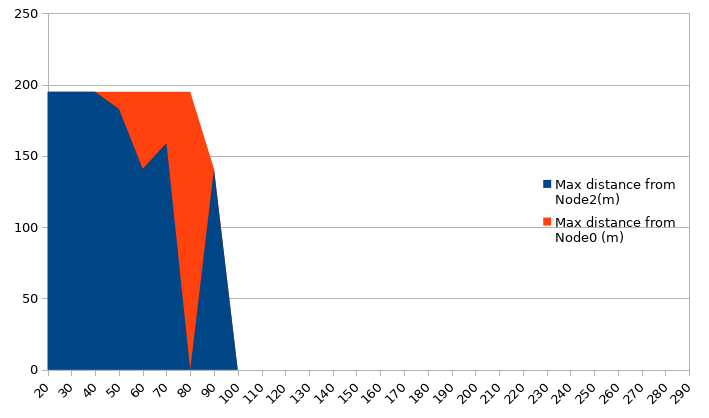
\includegraphics[scale=0.7]{graph1a.png}
		\caption{Relationship between the speed of Node1 and the maximum distance along the y axis between Node0 and Node1, for which transmission occurs.}
	\end{figure}
	
	\subsection{Tast 1B}
	
	Now we implement the Friis propagation loss model. It takes 3 parameters: frequency, which we are told to fix at 2.4 GHz, and System Loss and Minimum Loss, which we are leaving at 1 and 0 dB respectively. Recall that Friis model involves a relationship between the loss and the distance between nodes which is quadratic. I.e. the loss is proportional to the square of the distance. 
	
	It is done by replacing the three lines starting at line 459 with the following:\\	
	\texttt{std::string lossModel = "ns3::FriisPropagationLossModel");}\\
	\texttt{std::string atr1 = "Frequency";}\\
	\texttt{wifiChannel.AddPropagationLoss (lossModel, atr1, DoubleValue(2400000000)); //2.4 GHz = 2400000000 Hz}
	
	The maximum distance away from Node0 and Node2 as a function of speed of Node1 is shown in Fig. 2.s
	
	\begin{figure}[h]
		\centering
		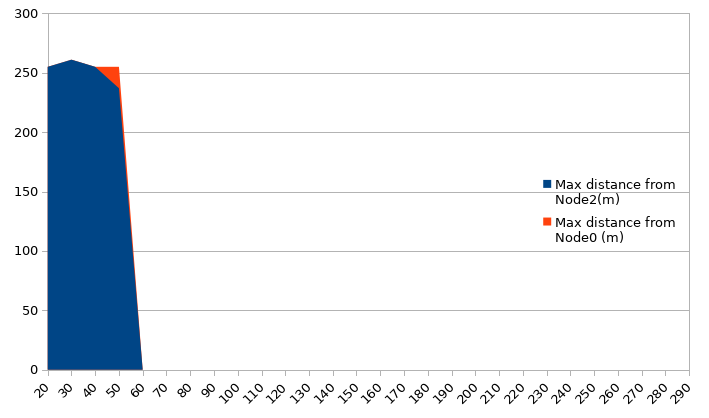
\includegraphics[scale=0.7]{graph1b.png}
		\caption{Relationship between the speed of Node1 and the maximum distance along the y axis between Node0 and Node1, for which transmission occurs.}
	\end{figure}
	
	\subsection{Task 2A}
	
	To count the number of mails received at Node2, we introduce a global variable, \texttt{Number\_mails\_rcvd\_at\_node2} at the start of the program, and set it to 0. Then in the \texttt{Node2ReceivePacket(...)} function we update it after parsing the message:
	
	\texttt{Number\_mails\_rcvd\_at\_node2 += receivedpacket\_head - (receivedpacket\_tail - 1)} 
	
	And add it to the logging: 
	
	\texttt{std::cout << "The total number of mails received so far is " << Number\_mails\_rcvd\_at\_node2 << std::endl;}
	
	The results are as shown in Fig. 4. Throughout the simulation, we consistently receive 1 packet, regardless of the speed of Node1 and distance from Node0, up to the transmission limits shown before. While disappointing, it is understandable, once we inspect contents of the Node1's buffer at each point. 
	
	Node0 sends its data across every 0.25 s, while generating a new message every second. So it first sends its message 1, receives acknowledgement from Node1, purges its buffer, and then creates message number 2, which is now the only message in the buffer.
	
	Meanwhile Node1 keeps replacing the content of its own buffer with the packet received from Node0. Each of these packets contain only a single message, and so Node1's buffer can contain at most 1 message at a time in this scenario. Thus there's only one message sent to Node2 in each iteration.
	
	\begin{figure}[h]
		\centering
		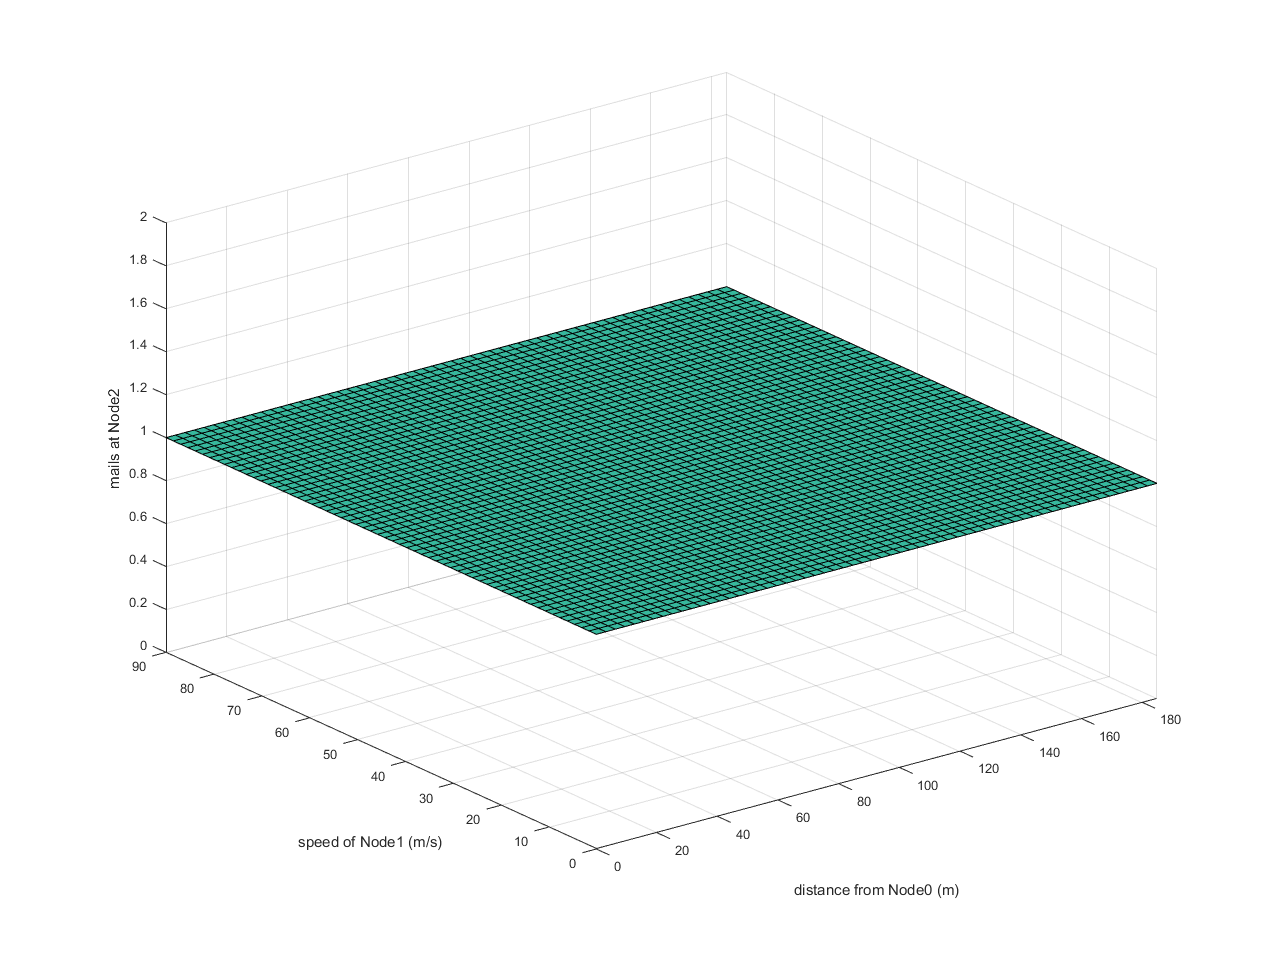
\includegraphics[scale=0.4]{graph2a.png}
		\caption{Number of packets received at Node2}
	\end{figure}
	\pagebreak
	\subsection{Task 2B}
	
	First note that in order to keep all messages in the buffer, we should not simply store the value  of the tail from the first data packet we receive, and keep updating the head. It is possible that we do not receive all messages between them. For example we may receive the first buffer load of Node0 with messages 1, 2, and 3, and the next packet may contain messages 5, 6, and 7. Thus we don't get message number 4, while keeping only one tail and head would imply otherwise. However in this simple simulation, this will not cause problems.
	
	This was tested by logging the contents of each packet received by Node1.
	
	Thus, we update Node1's tail only once, with the first packet received. To this end we survive 342 with an if statement:\\
	\tab\texttt{if (Pkt\_no\_last\_seen\_by\_node1 == 0) \{ }\\
	\tab\tab \texttt{node1\_tail = header.Gettail();}\\
	\tab\texttt{\}}
	
	We also need to make sure that we update the variable \texttt{Pkt\_no\_last\_seen\_by\_node1} after that if statement, so we simply move line 334 further down.
	
	This time we can clearly see the number of messages decreasing as both speed of Node1 and distance from Node0 increases, because Node1 leaves the transmission range of Node0 quicker.	
	
	\begin{figure}[h]
		\centering
		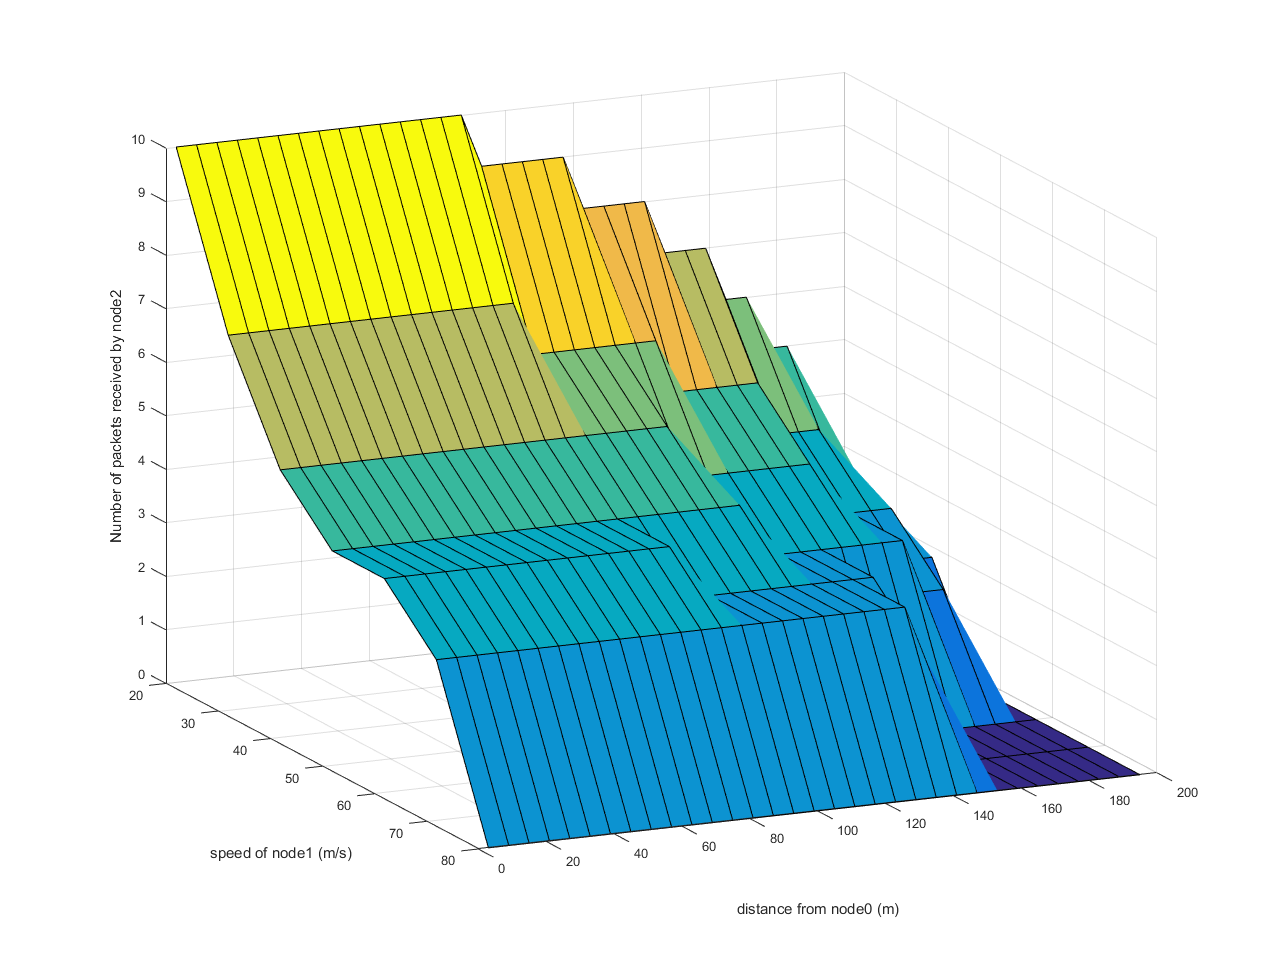
\includegraphics[scale=0.4]{graph2b.png}
		\caption{Number of packets received at Node2}
	\end{figure}
	
	\pagebreak
	\subsection{Task 3A}
	
	To add a second mobile node, there are multiple places in the code where changes have to be made. Firstly we copy all higher level code for Node1 and change it to be about the new Node3. This also includes adding a couple of variables such as \texttt{Node3Ack} or \texttt{node3\_head}. Then we increase the total number of nodes defined on line 551\footnote{line numbers referring to file \texttt{CS345finproj3.cc}}, and add it to the container of mobile nodes. We set the position, velocity and mobility model in the same fashion as we do for Node1. The position should be set to \texttt{Vector(-250.0, distance\_between\_node0\_node1, 0.0)}.
	
	We also need to connect Node3 to Node0 and Node2. It is important to note that especially Node2 cannot be in multicast mode, because then when it sends an acknowledgement for a packet received from Node1, Node3 will also pick that acknowledgement and stop sending. To sort out this issue, we create two receiving sockets for Node2 and add a parameter to function \texttt{Node2ReceivePacket}, which tells us which node the packet came from. Then each socket makes callback with a different parameter, and based on it we can send the acknowledgement directly to the relevant node. We also use this parameter for additional logging.
	
	Additionally we have to increase the duration of the simulation to say 505 s, so that Node3 has time to reach Node2, and change how we calculate the total number of unique mails seen at Node2.
	
	\section{Concluding remarks}
	
	We have simulated a delay tolerant network. They have their uses in real life, for example in tracking movement of animals, by fitting them with a GPS sensor and a transceiver, which then transmits its data whenever they came in range of a stationary node, or in smart cars, which communicate with e.g. cellular network stations. 
	
	We discovered that in general the reliability and robustness of the transmission decreases with the distance from the stationary nodes, and with the speed of mobile nodes.
	
	However, it is worth noting, that we started our simulation at 20 m/s which is 72 km/h - a realistic speed of a car travelling between urban areas. The speed reached in the simulations are closer to a speed of 360 km/h, which the speed of an F1 car, and much faster than any average ground vehicle (or animal) can achieve in a realistic situation (we are not talking about speed tests on a race circuit after all).
	
	It has to be pointed out though that we are not using a realistic propagation loss model, and to make it closer to reality, we should be using log-distance or Friis. There are also other tweaks that can be made to reflect real life situations better.
	
	\pagebreak
	\begin{thebibliography}{1}
		\bibitem{range loss doc}
		Range Propagation Loss Model, NS-3 documentation, available online: \url{https://www.nsnam.org/doxygen/classns3_1_1_range_propagation_loss_model.html}
	\end{thebibliography}
	% that's all folks
\end{document}

